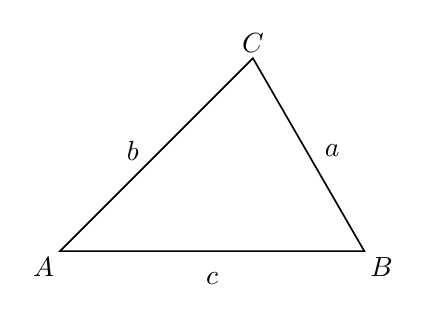
\begin{tikzpicture}[x=1cm,y=1cm,font=\normalsize,
 geometry edge/.style={solid,line width=.6pt},
 geometry mark/.style={solid,line width=.6pt},
 geometry label/.style={font=\normalsize,inner sep=2pt}]
\coordinate (A) at (0,0);
\coordinate (B) at (3.863703,0);
\coordinate (C) at (2.44949,2.44949);
\draw[geometry edge] (A)--(B)--(C)--cycle;
\node[font=\normalsize,inner sep=2pt] at (0.924745,1.274745) {$b$};
\node[font=\normalsize,inner sep=2pt] at (3.456597,1.274745) {$a$};
\node[font=\normalsize,inner sep=2pt] at (1.931852,-0.35) {$c$};
\node[geometry label,below left] at (A) {$A$};
\node[geometry label,below right] at (B) {$B$};
\node[geometry label,above] at (C) {$C$};
\end{tikzpicture}
